\clearpage
\section{Coupler 2 by 2}

In general, the matrix representing 2x2 coupler can be summarized in the following way,
\begin{equation}
\begin{bmatrix}
A' \\
B'
\end{bmatrix}=\begin{bmatrix}
  					T  & iR \\
					iR & T
			  \end{bmatrix} \dot{}{\begin{bmatrix}
			  				     A \\
			  	                 B
			  	                 \end{bmatrix}}
\end{equation}
Where, A and B represent inputs to the 2x2 coupler and A' and B' represent output of the 2x2 coupler. Parameters T and R represent transmitted and reflected part respectively which can be quantified in the following form,

\begin{equation}
T=\sqrt{1-\eta_{R}}
\end{equation}

\begin{equation}
R=\sqrt{\eta_{R}}
\end{equation}
Where, value of the $\sqrt{\eta_{R}}$ lies in the range of $0 \leq \sqrt{\eta_{R}} \leq 1$.
\begin{figure}
	\centering
	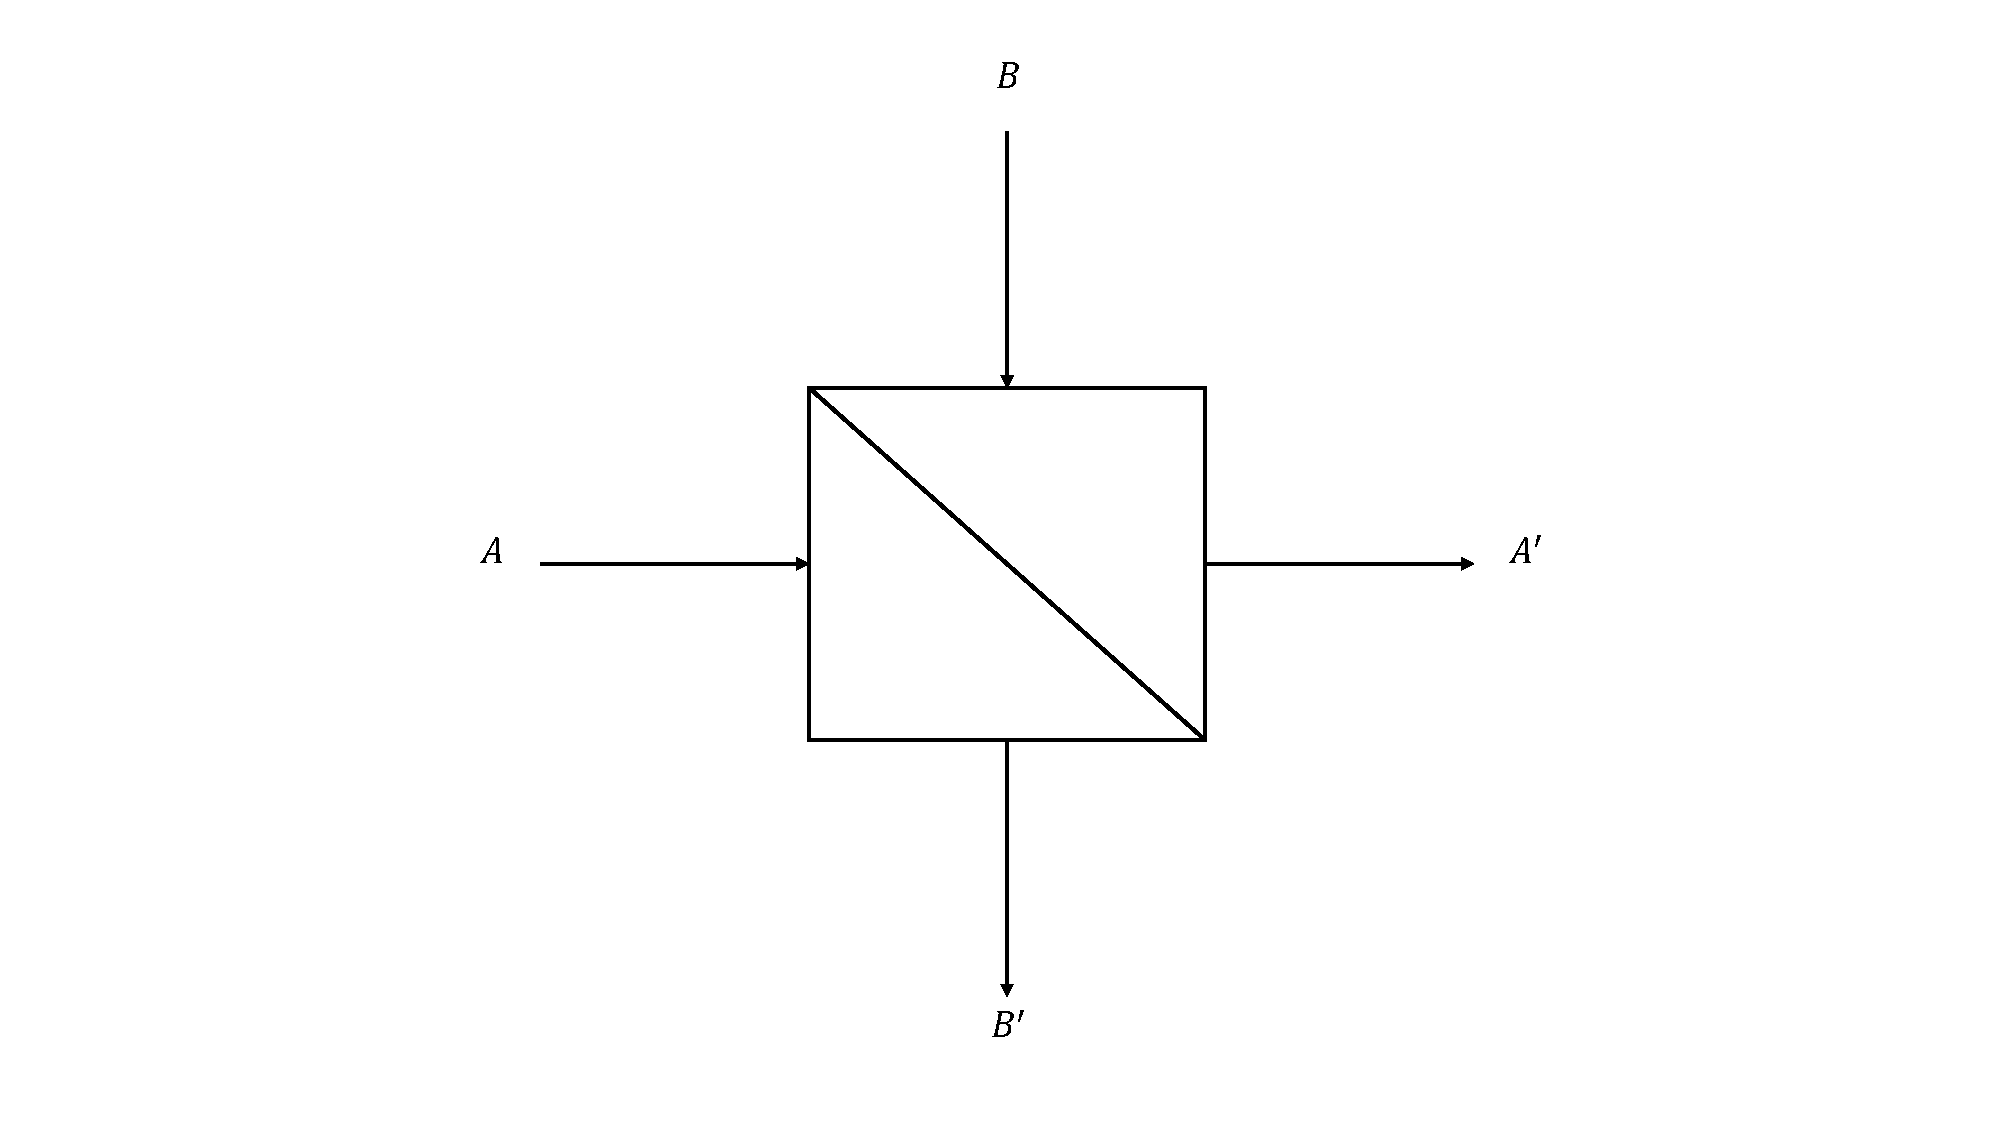
\includegraphics[width=\textwidth]{./lib/coupler_2_by_2/figures/coupler_2_by_2.pdf}
	\caption{2x2 coupler}\label{}
\end{figure}

It is worth to mention that if we put $\eta_{R}=1/2$ then it leads to a special case of "Balanced Beam splitter" which equally distribute the input power into both output ports.
